\section{A firewall analysis assistant in miniKanren}\label{firewall}
\subsection{Our simplified model}
There are many types of firewalls, but for this work we will only consider networking firewalls defined by Access Control Lists (ACL). An ACL is a sequence of entries, each in turns defines a range of values to be compared against network packets. When an ACL processes a packet, it compares the packet against its entries from top to bottom until a matched entry is found, and an action specified by that entry is taken. For our purpose, we assume that actions can only be either \textit{permit} or \textit{deny}, the meaning of which will depend on the practical context.

Modeling is the most important aspect of this work. Although there is practical value in models that are close to how real life ACL works, they are not very simple to understand and to work with. Therefore, in this paper we will construct our own model simple enough to demonstrate the fundamental ideas.

In our model, a packet is simply a quadruple of values belonging to four fields: its protocol, its source address, its destination address and its flag. Correspondingly there are three high-level ranges (types of values):
\begin{itemize}
    \item \textbf{All protocols} (Denoted \code{*p}): A protocol is a specific format of data such as \code{tcp}, \code{udp}, \code{icmp}, etc.
    \item \textbf{All addresses} (Denoted \code{*a}): Although IPv4 addresses are predominantly used these days, we will assign symbolic values for addresses for simplicity. Examples can be \code{pc-a}, \code{isp}, etc.
    \item \textbf{All flags} (Denoted \code{*e}): A flag is a TCP field to determine the connection phase. There are only two Boolean values \code{#t} (established) and \code{#f} (not established).
\end{itemize}

There is actually a hierarchy of ranges to help in configuring ACL. The example hierarchy in figure \ref{hier} is global in this paper, but it can be customized depending on the specific use case (especially the addresses).

\begin{figure}
    {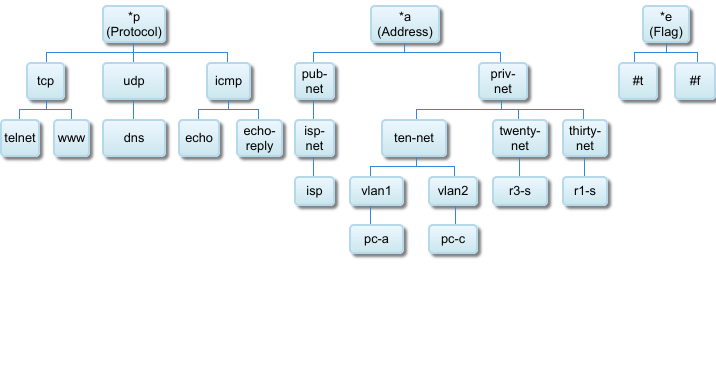
\includegraphics[width=\textwidth]
    {figures/hier.png}}
    \caption{\label{hier} Hierarchy of ranges}
\end{figure}

Values are leaves at the bottom of the trees. Note that even though all values are ranges, but some ranges are not necessarily values. Additionally, this data can be nicely translated to S-expression\footnote{This expressions is a \textit{forest}, which in turns is a list of \textit{trees}. We will describe trees and forests later on the in the implementation.}:
\begin{lstlisting}
((*p (tcp (telnet) (www))
     (udp (dns))
     (icmp (echo) (echo-reply)))
     
 (*a (pub-net  (isp-net (isp)))
     (priv-net (ten-net (vlan1 (pc-a))
                        (vlan2 (pc-c)))
               (twenty-net (r3-s))
               (thirty-net (r1-s))))
               
 (*e (#t) (#f)))
\end{lstlisting}

\subsection{Implementation of the firewall analyzer}
With the model in mind, we can translate each concept into its representation as S-expressions. A packet is a list of its values of the four fields (e.g. \code{(telnet isp isp #t)}). ACLs are lists of their entries. An entry is like a packet, but with ranges instead of values for its fields and an action attached to the beginning. For example, \code{(deny *p *a *a *e)} is the familiar "deny all" entry inserted implicitly at the end of each ACL. That much can help us define the first two high-level functions \code{entry-matcht} and \code{acl-mapo}. \code{entry-matcht} is a pseudo-function of \code{entry} and \code{pkt} and returns the result of the question "Does \code{pkt} match \code{entry}?". \code{acl-mapo} uses \code{entry-matcht} to process the packet \code{pkt} with the entries in \code{acl} and unifies \code{entry} with the one that the packet matches. Due to the implicit "deny all" at the end, every packet will match with an entry as long as it is well-formed.
\begin{lstlisting}
(define entry-matcht
  (lambda (entry pkt)
    (lambda (?)
      (fresh (eaction epkt)
        (== `(,eaction . ,epkt) entry)
        ((super*t epkt pkt) ?)))))

(define acl-mapo
  (lambda (acl pkt entry)
    (conde
     [(== '() acl)
      (== entry '[deny *p *a *a *e])
      (;; Ensures that the packet is well-formed
       (entry-matcht entry pkt)
       #t)]
     [(fresh (a d)
        (== `(,a . ,d) acl)
        (condo
         [(entry-matcht a pkt) (== a entry)]
         [else (acl-mapo d pkt entry)]))])))
\end{lstlisting}

To ask if a packet matches an entry is a question of determining whether the ranges in the entry cover the values in the packet. Therefore, the hierarchy in figure \ref{hier} is involved and for that we need \textbf{tree} processing. Trees are formally defined as the mutually recursive data structure where:
\begin{itemize}
    \item A tree is a pair of an arbitrary value (its \textbf{root node}) and a forest (its \textbf{children}) and
    \item A forest is a list of trees.
\end{itemize}

\begin{figure}
    {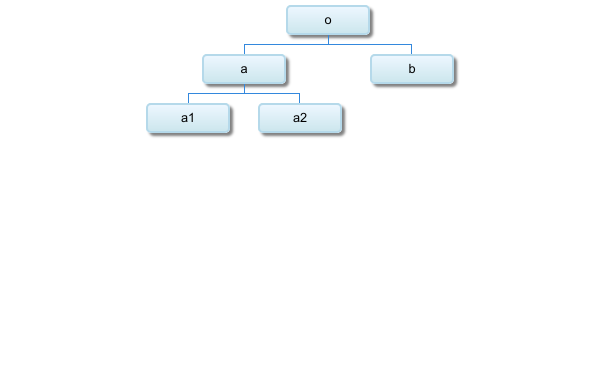
\includegraphics[width=\textwidth]
    {figures/example-tree.png}}
    \caption{\label{example-tree} Example tree}
\end{figure}

For instance, the tree in figure \ref{example-tree} is written in S-expression as \code{(o (a (a1) (a2)) (b))}. We define the tree find and forest find relations below. These two are also pseudo-functions because they need to communicate internally whether \code{sub} is found under a \code{tree} or \code{forest}.
\begin{lstlisting}
(define tree-forest-findt
  (lambda (sub)
    (letrec
        ([tree-findt
          (lambda (tree)
            (lambda (found?)
              (fresh (v u f g)
                (== tree `(,v . ,f))
                (== sub  `(,u . ,g))
                (condo
                 [(==t u v)
                  (== f g)
                  (== #t found?)]
                 [else
                  ((forest-findt f) found?)]))))]

         [forest-findt
          (lambda (forest)
            (lambda (found?)
              (conde
               [(== '() forest) (== #f found?)]
               [(fresh (a d)
                  (== `(,a . ,d) forest)
                  (condo
                   [(tree-findt a) (== #t found?)]
                   [else ((forest-findt d) found?)]))])))])

      (values tree-findt forest-findt))))

(define tree-findt
  (lambda (tree sub)
    (let-values ([(t _f) (tree-forest-findt sub)])
      (t tree))))

(define forest-findt
  (lambda (forest sub)
    (let-values ([(_t f) (tree-forest-findt sub)])
      (f forest))))
\end{lstlisting}

Finally, we define the relations to represent when a range subsumes a value. \code{supert} is the core, dealing with a single field. It finds the subtree with root \code{v1} in the hierarchy (which is always successful) and then find the leaf node \code{v2} under that subtree, the result of which is the result of the entire function. \code{super*t}, used by \code{entry-matcht} above, handles all four fields\footnote{However, \code{super*t} is defined on arbitrary lists so it can handle infinitely many fields should we want it to.}.
\begin{lstlisting}
(define supert
  (lambda (v1 v2)
    (lambda (?)
      (fresh (t1 _f1)
        (== t1 `(,v1 . ,_f1))
        ((forest-findt hier t1)     #t)
        ((tree-findt   t1   `(,v2)) ?)))))

(define super*t
  (lambda (e1 e2)
    (lambda (?)
      (conde
       [(== '() e1) (== '() e2) (== #t ?)]
       [(fresh (a1 d1 a2 d2)
          (== `(,a1 . ,d1) e1)
          (== `(,a2 . ,d2) e2)
          ((conjt (supert a1 a2)
                  (super*t d1 d2))
           ?))]))))
\end{lstlisting}

\subsection{Sample usage}
Our examples use the ACL below:
\begin{lstlisting}
(define acl100
  '([permit www  ten-net *a         *e]
    [permit tcp  pc-a    r3-s       *e]
    [deny   echo ten-net twenty-net *e]
    [permit icmp ten-net twenty-net *e]))
\end{lstlisting}

Given a packet \code{[echo pc-a r3-s #f]}, we can ask the question "Does acl100 block this packet?" with this query:
\begin{lstlisting}
(let ([pkt '[echo pc-a r3-s #f]])
      (run* (entry)
        (acl-mapo acl100 pkt entry)))
\end{lstlisting}
$\Rightarrow$ \code{((deny echo ten-net twenty-net *e))}

The matched entry is a deny, so indeed it was blocked. This is, however, not an exciting example because we can do the same thing with Packet Tracer. The interesting examples come from running the programs "backward". For example, we can ask which packets are blocked by acl100 (and by which entries):
\begin{lstlisting}
(run 10 (pkt entry)
      (fresh (?) (== `(deny . ,?) entry))
      (acl-mapo acl100 pkt entry))
\end{lstlisting}
$\Rightarrow$
\begin{lstlisting}
(((www isp isp #t)    (deny *p *a *a *e))
 ((www isp isp #f)    (deny *p *a *a *e))
 ((echo pc-a r3-s #t) (deny echo ten-net twenty-net *e))
 ((echo pc-a r3-s #f) (deny echo ten-net twenty-net *e))
 ((echo pc-c r3-s #t) (deny echo ten-net twenty-net *e))
 ((echo pc-c r3-s #f) (deny echo ten-net twenty-net *e))
 ((www isp pc-a #t)   (deny *p *a *a *e))
 ((www isp pc-a #f)   (deny *p *a *a *e))
 ((www isp pc-c #t)   (deny *p *a *a *e))
 ((www isp pc-c #f)   (deny *p *a *a *e)))
\end{lstlisting}

How to read this: packet \code{(www isp isp #t)} is blocked by the "deny all" entry, packet \code{(echo pc-a r3-s #t)} is blocked by the \code{(deny echo ten-net twenty-net *e)} entry, etc. Although the program works as expected, we found a glaring issue that even non-TCP packets can contain the established flag. I think fixing this should be easy, but chose not to do so for the simplicity of the code.

By restricting the entry parameter even more, we question the usefulness of each entry. For example, we can ask which function the final entry serves (if it even does anything).
\begin{lstlisting}
(run 1 (pkt entry)
  (fresh (?) (== '[permit icmp ten-net twenty-net *e] entry))
  (acl-mapo acl100 pkt entry))
\end{lstlisting}
$\Rightarrow$
\begin{lstlisting}
(((echo-reply pc-a r3-s #t)
  (permit icmp ten-net twenty-net *e)))
\end{lstlisting}

For the grand finale, we can ask the computer to synthesize an entry, given a specified behavior:
\begin{lstlisting}
(run 1 (missing)
      (fresh (acl e1 e2)
        (== `([permit www  ten-net *a         *e]
             [permit tcp  pc-a    r3-s       *e]
             ,missing
             [permit icmp ten-net twenty-net *e])
           acl)
        (fresh (?) (== `(deny . ,?)   e1))
        (fresh (?) (== `(permit . ,?) e2))
        (acl-mapo acl '[echo       pc-a r3-s #f] e1)
        (acl-mapo acl '[echo-reply pc-a r3-s #f] e2)))
\end{lstlisting}
And... miniKanren never returns an answer, at least with today's hardware.